\documentclass[a4paper]{article}

\usepackage{ctex}
\usepackage{amsmath}
\usepackage{float}
\usepackage{subfigure}
\usepackage{graphicx}
\usepackage{appendix}

\usepackage{booktabs}
\usepackage{color,xcolor}
\usepackage{textcomp}
\usepackage{listings}
%\usepackage[utf8]{inputenc}
\bibliographystyle{plain}



\title{基于层次分析法下的旅游地选择}
\date{}

\begin{document}
    \maketitle
    \begin{abstract}
        在当今学子高考毕业后,往往有着一个漫长的假期来供自己所支配,在这之中便有一些人选择了旅游。而本文便采取了层次分析法来进行相关的分析与研究。该问题的研究可以为高考毕业后想要去旅游的学子提供一个参考性意见。
        \\
        
        在这个问题中我们采取了层次分析法进行相关的研究,对此我们最后挑出了景色、花费、居住、饮食和交通等五个因素来对苏杭、北戴河和桂林等地进行分析,最后我们得到的结论是,忽略一切外部非客观条件,最终对于小明,旅游地的选择顺序是 桂林 > 苏杭 > 北戴河。
        \\
         
        最后,本文对该模型的优、缺点进行了评价及模型推广,得出该模型还可以在高考后志愿的选择等问题上进行再一步的研究。\vspace{250pt}
        \\
        \textbf{关键词:}毕业学子的旅游地选择\quad 层次分析法
    \end{abstract}
    
    \newpage 
    \section{问题的重述}
    在高考完之后,小明打算利用这个假期去外旅游,经过一系列的筛选之后,小明初步确定了三个目的地来供选择,它们分别是苏杭、北戴河和桂林。但是小明却对这三个目的地最终去哪而感到抓狂。请你通过相关的分析、研究来为小明确定最终旅游的目的地。
    \section{模型的假设}
    \begin{enumerate}
        \item 假设旅游的预算充足。
        \item 假设目的地的天气等客观条件都良好。
        \item 无其它主观因素
    \end{enumerate}
    \section{符号说明}
%    
%    \begin{table}[h]
%    \centering
%    \caption{符号说明}
%    \label{tab:}
%    \begin{tabular}{@{}lclllcl@{}}
%    \toprule
%     & 符号 &  &  &  & 说明       &  \\ \midrule
%     & O  &  &  &  & 目标层      &  \\
%     & R  &  &  &  & 准则层      &  \\
%     & c  &  &  &  & c色hi是    &  \\
%     & S  &  &  &  & 是DVD VS的 &  \\ \bottomrule
%    \end{tabular}
%    \end{table}
    \begin{table}[h]
    \centering
    \caption{符号说明}
    \begin{tabular}{cc}
    \toprule[1.5pt]
    \makebox[0.3\textwidth][c]{符号}&\makebox[0.4\textwidth][c]{说明}\\
    \midrule
    $  O $ & 目标层\\
    $ M $ & 准则层\\
    $ P $ & 方案层\\
    $ \lambda_{max}$&最大特征值\\
    $ \omega $ & 权重\\
    $ CI $ & 一致性指标\\
    $ RI $ & 一致性比例\\    
    \bottomrule[1.5pt]
    \end{tabular}
    \end{table}
    \section{模型的建立与求解}
    \subsection{问题分析}
    由于题目中并没有给出明确的数据支持,且针对此问题也具有着很多的影响因素,所以我们通过询问相关专家及上网查询\cite{__2012},最终确定了景色、花费、居住、饮食和交通等五个因素来进行相关研究。
%    \subsection{层次分析法的原理}
%    层次分析法是由美国运筹学家 Saaty上世纪70年代创立的一种系统分析与决策的综合评价方法,是建立于人类思维过程的基础上从而提出来的,它较合理的解决了定性问题定量化的处理过程。
    \subsection{层次分析法构建评价体系}

    \subsubsection{建立层次分析结构模型}
    将决策问题分为三个层次:最上层为目标层$O$,即选择最合适的旅游地;中间层为准则层$M$,即景色$M_{1}$、花费$M_{2}$、居住$M_{3}$、饮食$M_{4}$和交通$M_{5}$五个指标;最后一层为方案层,即对于苏杭$P_{1}$、北戴河$P_{2}$和桂林$P_{3}$的选择,如图所示:
    \begin{figure}[H]
    \centering
    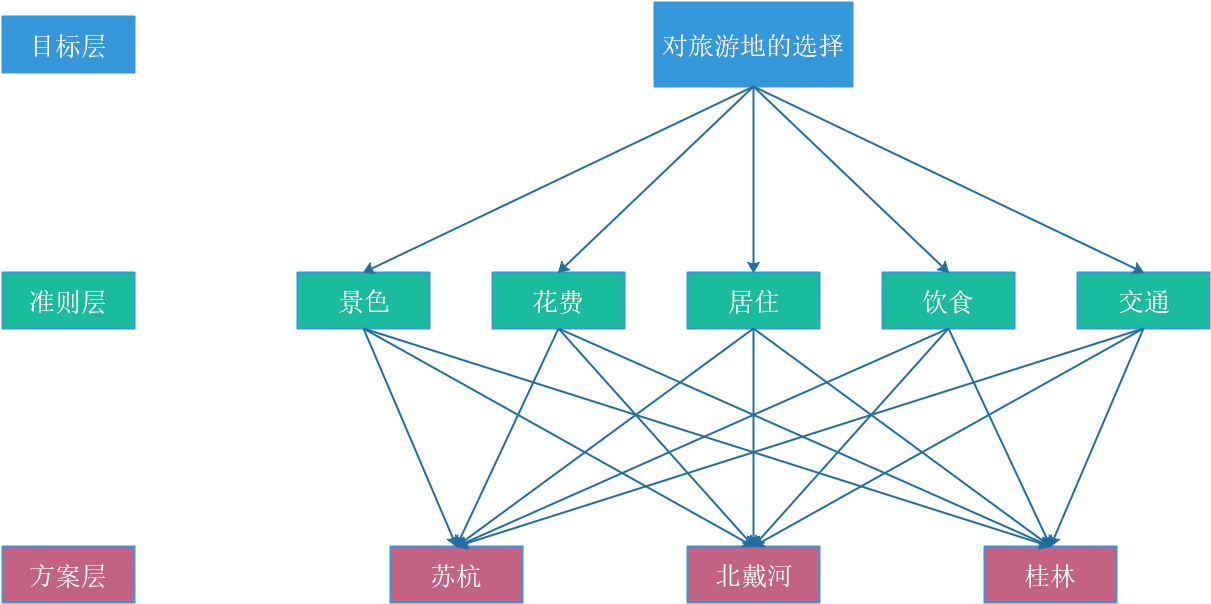
\includegraphics[width=0.8\linewidth]{fig/AHP}
    \caption{层次分析图示}
    \label{fig:ahp}
    \end{figure}
    \subsubsection{模型求解}
    $ \left( 1\right) $ 构造判断矩阵$O-M$:将准则层的五个元素通过专家询问等方式两两进行比较,得到判断矩阵,如表二所示:
    \begin{table}[H]
    \centering
    \caption{$ O-M $判断矩阵}
    \label{tab:my-table}
    \begin{tabular}{@{}cccccc@{}}
    \toprule
       & 景色  & 花费  & 居住 & 饮食  & 交通  \\ \midrule
    景色 & 1   & 1/2 & 4  & 3   & 3   \\
    花费 & 2   & 1   & 7  & 5   & 5   \\
    居住 & 1/4 & 1/7 & 1  & 1/2 & 1/3 \\ 
    饮食 & 1/3 & 1/5 & 2  & 1   & 1   \\ 
    交通 & 1/3 & 1/5 & 3  & 1   & 1   \\ \bottomrule
    \end{tabular}
    \end{table}
    简单计算可得上述$ O-M $判断矩阵的$ \lambda_{max} $为5.071,且权重向量$ \omega_{i}$为$\left( 0.263,0.475,0.053,0.098,0.108\right) $由公式 $CI=\dfrac{\lambda _{\max}-1}{n-1} $及$CR=\dfrac{CI}{RI}$,计算得到$ CR = 0.01609 < 0.1 $通过了一致性检验。
    \begin{table}[H]
    \centering
    \caption{平均随机一致性指标$ RI $}
    \begin{tabular}{|c|c|c|c|c|c|c|c|c|}
    \hline
    n  & ~1~ & ~2~  & 3    & 4    & 5    & 6    & 7    & 8    \\ \hline
    RI & ~0~ & ~0~  & 0.58 & 0.90 & 1.12 & 1.24 & 1.32 & 1.41 \\ \hline
    \end{tabular}
    \end{table}
    $ \left( 2\right)  $构建判断矩阵~:\\
    \begin{minipage}{\textwidth}
        \begin{minipage}[H]{0.5\linewidth}
            \centering
            \begin{table}[H]
                \centering
                \caption{$ M_{1}-P $判断矩阵}
                \begin{tabular}{|c|c|c|c|}
                    \hline
                    景色  & 苏杭  & 北戴河 & 桂林 \\ \hline
                    苏杭  & 1   & 2   & 5  \\ \hline
                    北戴河 & 1/2 & 1   & 2  \\ \hline
                    桂林  & 1/5 & 1/2 & 1  \\ \hline
                \end{tabular}
            \end{table}
        \end{minipage}
        \begin{minipage}[H]{0.5\linewidth}
            \centering
            \begin{table}[H]
                \centering
                \caption{$ M_{2}-P $判断矩阵}
                \begin{tabular}{|c|c|c|c|}
                    \hline
                    花费  & 苏杭 & 北戴河 & 桂林  \\ \hline
                    苏杭  & 1  & 1/3 & 1/8 \\ \hline
                    北戴河 & 3  & 1   & 1/3 \\ \hline
                    桂林  & 8  & 3   & 1   \\ \hline
                \end{tabular}
            \end{table}
        \end{minipage}
    \end{minipage}
    \begin{minipage}{\textwidth}
        \begin{minipage}[H]{0.5\linewidth}
            \centering
            \begin{table}[H]
                \centering
                \caption{$ M_{3}-P $判断矩阵}
                \begin{tabular}{|c|c|c|c|}
                    \hline
                    居住  & 苏杭  & 北戴河 & 桂林 \\ \hline
                    苏杭  & 1   & 1   & 3  \\ \hline
                    北戴河 & 1   & 1   & 3  \\ \hline
                    桂林  & 1/3 & 1/3 & 1  \\ \hline
                \end{tabular}
            \end{table}
        \end{minipage}
        \begin{minipage}[H]{0.5\linewidth}
            \centering
            \begin{table}[H]
                \centering
                \caption{$ M_{4}-P $判断矩阵}
                \begin{tabular}{|c|c|c|c|}
                    \hline
                    饮食  & 苏杭  & 北戴河 & 桂林 \\ \hline
                    苏杭  & 1   & 3   & 4  \\ \hline
                    北戴河 & 1/3 & 1   & 4  \\ \hline
                    桂林  & 1/4 & 4   & 1  \\ \hline
                \end{tabular}
            \end{table}
        \end{minipage}
    \end{minipage}
    \begin{table}[H]
        \centering
        \caption{$ M_{5}-P $判断矩阵}
        \begin{tabular}{|c|c|c|c|}
            \hline
            交通  & 苏杭 & 北戴河 & 桂林  \\ \hline
            苏杭  & 1  & 1   & 1/4 \\ \hline
            北戴河 & 1  & 1   & 1/4 \\ \hline
            桂林  & 4  & 4   & 1   \\ \hline
        \end{tabular}
    \end{table}
    同样,经过一致性检验,得到它们的$ CR $结果如下表所示: 
    \begin{table}[H]
        \centering
        \caption{ $ CR_{i} $计算结果}
        \begin{tabular}{@{}cccccc@{}}
          \toprule
          $ CR_{1} $ &  $ CR_{2} $ &  $ CR_{3} $ &  $ CR_{4} $ & $ CR_{5} $ \\ \midrule
            0.0053222 & 0.0014823 & 0.00 & 0.0088488 & 0.00 \\ 
          \bottomrule
        \end{tabular}
    \end{table}
    从上表中我们可以看出矩阵$ M_{i}-P $都通过了一致性检验。
    \subsubsection{模型结果与分析}
    根据上述数据,我们最终计算出$ M $层的各个影响因素所占的总权重,并汇总至下表:
    \begin{table}[H]
        \centering
        \caption{权重矩阵}
        \begin{tabular}{@{}ccccc@{}}
            \toprule
            & 指标权重   & 苏杭     & 北戴河    & 桂林     \\ \midrule
            景色 & 0.2636 & 0.5954 & 0.2764 & 0.1283 \\
            花费 & 0.4758 & 0.0819 & 0.2363 & 0.6817 \\
            居住 & 0.0538 & 0.4286 & 0.4286 & 0.1429 \\
            饮食 & 0.0981 & 0.6337 & 0.1919 & 0.1744 \\
            交通 & 0.1087 & 0.1667 & 0.1667 & 0.6667 \\\bottomrule
        \end{tabular}
    \end{table}
    根据上面的权重表,我们计算出了三个目的地的最终得分:
    \begin{table}[H]
        \centering
        \caption{最终得分表}
        \label{tab:my-table}
        \begin{tabular}{@{}cccc@{}}
            \toprule
            旅游地 & 苏杭    & 北戴河   & 桂林    \\ \midrule
            得分  & 0.299 & 0.245 & 0.455 \\ \bottomrule
        \end{tabular}
    \end{table}
    由上表可知,最终旅游地的选择顺序是~桂林 > 苏杭 > 北戴河 。
    \section{模型的评价与推广}
    \subsection{模型的评价与优化}
    \subsubsection{层次分析法的评价}
    层次分析法它较合理地解决了定性问题定量化的处理过程。它体现了人类决策思维的基本特征,即分解、判断、综合,克服了其他方法回避决策者主观判断的缺点,保证了了决策的有效性、可靠性和可行性\cite{司守奎}。
    \subsubsection{在此例中的优化}
    我们发现,在上述权重的计算当中,我们只采用了一种方法,对此我们可以采取多种方法计算然后取其平均值,这样可以更好的保证结果的稳健性,从而使得最终得出的结论更全面有效。详情请见附录A。
    \subsection{模型的推广}
    此种分析方法可以广泛的应用到生活中的方方面面,比如:高考后志愿的选择、大学生购买电脑时的比较等等。
    
    \bibliography{AHP}
    \newpage
    \appendix 

%        \section{层次分析法代码}
%        \lstinputlisting[language = matlab,keywordstyle=\color{blue!70}, commentstyle=\color{red!50!green!50!blue!50}, escapeinside=``, basicstyle=\tiny]{./code/AHP.m}
    \section{权重的计算方法}
    \subsection{算术平均法}
    第一步: 将判断矩阵按照列归一化。(每一个元素除以其所在列的和)
    
    第二步: 将归一化的各列相加(按行求和) 
    
    第三步: 将相加后得到的向量中每个元素除以n即可得到权重向量。
    
    假设判断矩阵$ A= 
    \left| \begin{matrix}
        a_{11}&		a_{12}&		\cdots&		a_{1n}\\
        a_{21}&		a_{22}&		\cdots&		a_{2n}\\
        \vdots&		\vdots&		\ddots&		\vdots\\
        a_{n1}&		a_{n2}&		\cdots&		a_{nn}\\
    \end{matrix} \right|
    $,
    
    那么算术平均法求得的权重向量$ \omega_{i} = \dfrac{1}{n}\sum\limits_{j=1}^n{\dfrac{a{ij}}{\sum\limits_{k=1}^n{a_{kj}}}}\left( i\ =\ 1,2,\cdots ,n \right) 
    $
    \subsection{几何平均法}
    第一步: 将A的元素按照行相乘得到一个新的列向量。
    
    第二步: 将新的向量的每个分量开n次方。
    
    第三步: 对该列向量进行归一化即可得到权重向量。
    
    假设判断矩阵$ A= 
    \left| \begin{matrix}
        a_{11}&		a_{12}&		\cdots&		a_{1n}\\
        a_{21}&		a_{22}&		\cdots&		a_{2n}\\
        \vdots&		\vdots&		\ddots&		\vdots\\
        a_{n1}&		a_{n2}&		\cdots&		a_{nn}\\
    \end{matrix} \right|
    $,
    
    那么几何平均法求得的权重向量$ \omega_{i} =
    \dfrac{\left( \prod\limits_{j=1}^n{a_{ij}} \right) ^{\frac{1}{n}}}{\sum\limits_{k=1}^n{\left( \prod\limits_{j=1}^n{a_{kj}} \right) ^{\frac{1}{n}}}}
    $

    \subsection{特征值法}
    第一步:求出矩阵A的最大特征值以及其对应的特征向量。
    
    第二步:对求出的特征向量进行归一化即可得到我们的权重。
    \section{层次分析法代码}
    \begin{lstlisting}[language = matlab,keywordstyle=\color{blue!70}, commentstyle=\color{red!50!green!50!blue!50}, basicstyle=\tiny]
% 设置输出格式
% format rat
% 运行前先清屏
clear ,clc;
% 层次分析法
disp("请输入一个方阵:");
ori_mat=input('ori_mat = ');
% 检查输入情况
% 假设输入的矩阵没有错误
errno = 0;
% 1 是否为方阵
[row ,col]=size(ori_mat);
if row ~= col
    errno = 1;
end

% 2 检验矩阵中是否有负数或零出现
if errno == 0 % 如果已经有错误出现就不再进行判断
    check_mat = ori_mat <= 0;
    no_zero_sum = sum(sum(check_mat));
    if no_zero_sum > 0
        errno = 2;
    end
end

% 3 检验所输入的矩阵是否为正互反矩阵
if errno == 0 % 如果已经有错误出现就不再进行判断
    % aij*aji = 1
    check_mat = ori_mat .* ori_mat';
    result_mat = check_mat ~= ones(row,col);
    result = sum(result_mat(:)) ~= 0;
    if result ~= 0
        errno = 3;
    end
end

% 4 检验矩阵行数是否超过了15 --- 因为后续要进行 RI 的判断
if errno == 0 % 如果已经有错误出现就不再进行判断
    if col >= 15
        errno = 4;
    end
end

% 5 要是矩阵只有一个元素,那将毫无意义
if errno == 0 % 如果已经有错误出现就不再进行判断
   if row == 1
       errno = 5;
   end
end

% 对错误码进行校验
if errno == 0 % 说明所输入的矩阵符合规则
    flag = 1;% 进行标志位的设置
    % 先进行一致性检验
    RI=[0 0.00001 0.52 0.89 1.12 1.26 1.36 1.41 1.46 1.49 1.52 1.54 1.56 1.58 1.59];
    % 由于一些原因所以把RI的第二个元素改为了一个接近与0的数 --- 防止分母为 0
    [V,D] = eig(ori_mat);
    % V --- 特征向量,
    % D --- 由特征值构成的对角矩阵
    max_eig = max(D(:));% 找到最大特征值
    CI = (max_eig - row)/(row - 1);% 求出一致性指标
    CR = CI/RI(row);% 一致性比例
    disp(['一致性指标 CI = ',num2str(CI)]);
    disp(['一致性比例 CR = ',num2str(CR)]);
    if CR < 0.1
        disp('通过一致性检验');
    else
        disp('未通过一致性检验,需要对一致性判断矩阵进行修改!')
        flag = 0;
    end
    
    if flag 
        % 三种方法计算权重
        
        % 1 算数平均法求权重
        col_sum = sum(ori_mat);% 求每一列的和
        check_mat = repmat(col_sum,row,1);% 构造以列和为扩展的新的矩阵
        ari_result = sum((ori_mat./check_mat),2)/row;% 进行归一化处理
        disp('算术平均法求权重的结果为:');
        disp(ari_result);
        
        % 2 几何平均法求权重
        temp_mat = prod(ori_mat,2);% 进行每一行元素的相乘
        check_mat = temp_mat.^(1/col);% 对所得到的数值进行开n次方
        geo_result = check_mat ./ sum(check_mat);% 归一化处理
        disp('几何平均法求权重的结果为:');
        disp(geo_result);
        
        % 3 特征值法求权重
        [Row ,Col] = find(D == max_eig ,1);% 找到最大特征值所在的行和列
        eig_result = V(:,Col)./sum(V(:,Col));% 进行归一化处理
        disp('特征值法求权重的结果为:');
        disp(eig_result);
    end
else
    if errno == 1
        disp('所输入的矩阵不是方阵')
    elseif errno == 2
        disp('所输入的矩阵中出现了负数')
    elseif errno == 3
        disp('所输入的矩阵不满足正互反矩阵的要求')
    elseif errno == 4
        disp('所输入的矩阵行数及列数超过了15,此种方法判断会出现错误')
    elseif errno == 5
        disp('所输入的矩阵中只有一个元素')
    end
    
    disp('请检查输入!');
end
% % 还原默认显示格式
% format short
        \end{lstlisting}

\end{document}